\subsection{FLOps Overview}\label{subsection:flops_overview}

\begin{figure}[H]
    \begin{adjustwidth}{-0.1\paperwidth}{-0.1\paperwidth}
        \centering
        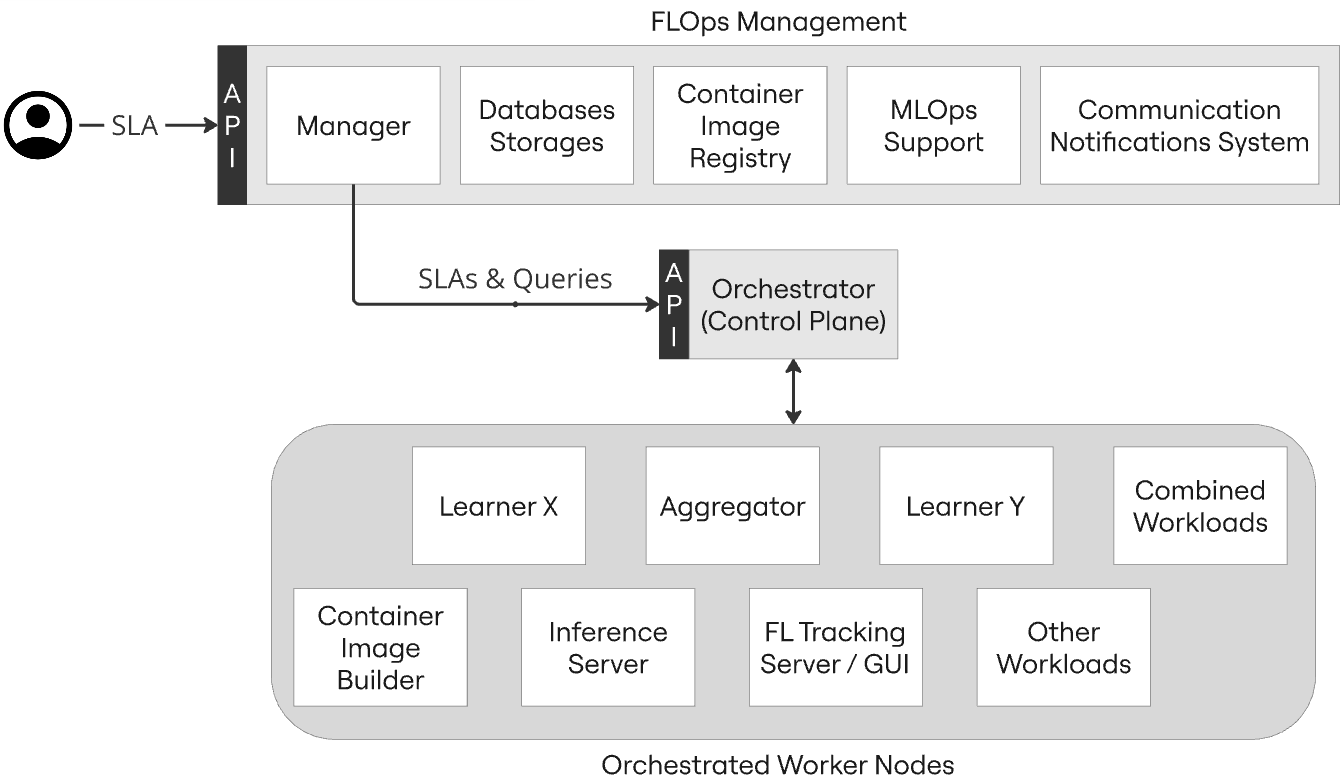
\includegraphics[width=0.8\paperwidth]{primer_flops.png}
        \caption{FLOps Structural Overview}
        \label{fig:flops_structure_overview}
    \end{adjustwidth}
\end{figure}

Figure \ref{fig:flops_structure_overview} provides a simplified overview of FLOps' structure.
Note that the management components and deployed services on orchestrated workers are interconnected.
These connections are not explicitly visualized to avoid clutter.
The services shown in the rounded rectangle depict an arbitrary number of worker nodes.
Multiple services can run on the same worker, or every worker might only have a single service deployed.
The FLOps system works via the interactions and relationships between the FLOps management, the orchestrator, and the worker nodes.
The FLOps management is a composition of components (containers).
Its goals and responsibilities are to manage FLOps processes and store FLOps artifacts.
The management components coordinate automatic processes and events.
They store container images and training results such as metrics and trained models.
These managerial components do not perform the FL training.
They delegate and distribute computation to orchestrated worker nodes.
The FLOps manager uses the orchestrator to create, (un)deploy, and remove different components.
The manager spreads computationally heavy image builds and FL training across the worker nodes.
The GUI and inference servers also run on worker nodes.

Figure \ref{fig:flops_simple_image_builder} shows a simplified overview of FLOps' image builder processes.
The container images get built on worker nodes.
Worker B stands for an arbitrary worker node capable of building images, i.e., the worker has enough resources and privileges.
The build process occurs inside a container that requires special considerations.
Remember that the user only provides ML code, not FL code.
FLOps' image builder clones the user ML code, augments it to support FL, handles specific dependency issues, and builds multi-platform container images.
This builder can build FL actors, i.e., the aggregator and learner images, as well as an inference server for the trained model.
These images get pushed to the FLOps image registry.
When the learners, aggregators, or inference servers are needed, their corresponding images are pulled from that registry onto an orchestrated worker node and executed.
Image builder services only exist when they are needed.
The FLOps manager removes them after building images for a concrete FLOps project.

\begin{figure}[h]
    \centering
    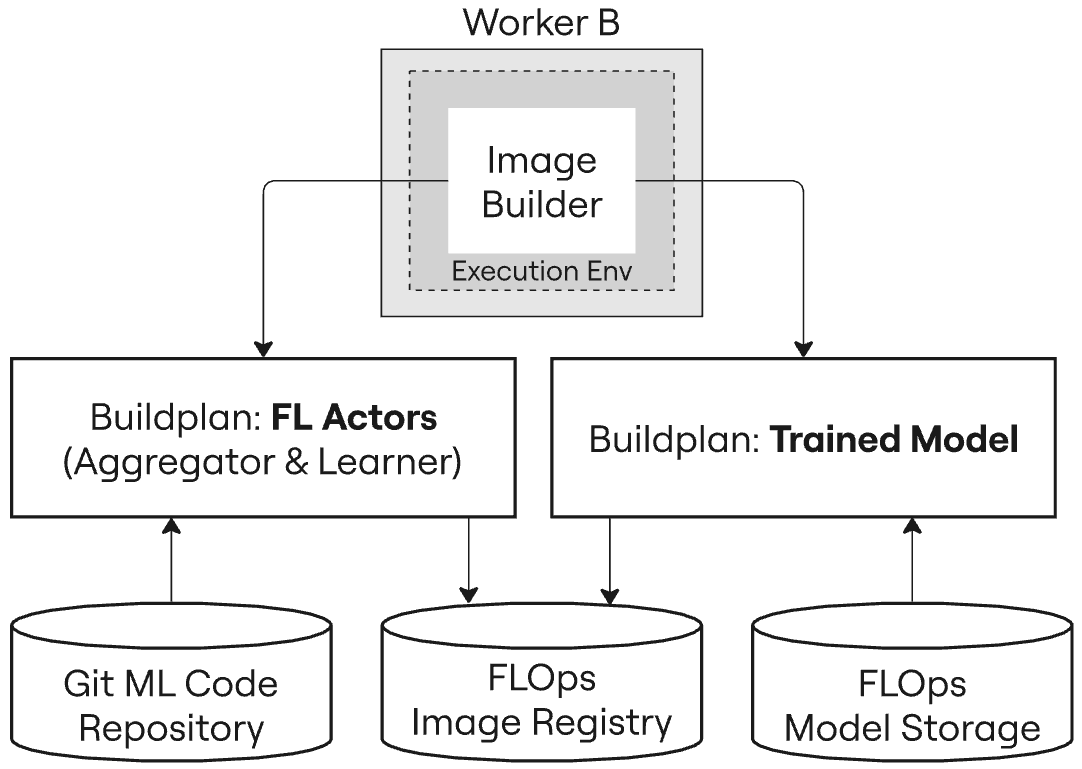
\includegraphics[width=0.8\textwidth]{simple_builder.png}
    \caption{Simplified FLOps Image Builder Processes}
    \label{fig:flops_simple_image_builder}
\end{figure}

\begin{figure}[H]
    \begin{adjustwidth}{-0.1\paperwidth}{-0.1\paperwidth}
        \centering
        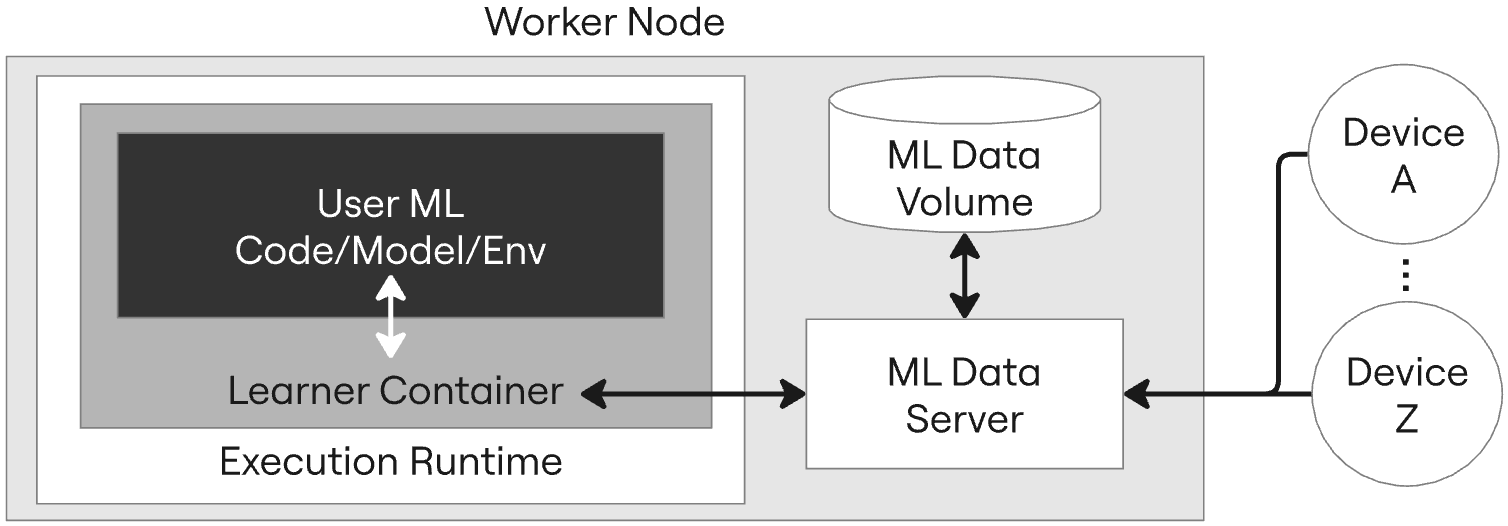
\includegraphics[width=0.70\paperwidth]{simple_data_management.png}
        \caption{Simplified FLOps Local Data Management}
        \label{fig:flops_simple_data_management}
    \end{adjustwidth}
\end{figure}

Figure \ref{fig:flops_simple_data_management} shows a simplified overview of how FLOps manages local training data.
FLOps targets practical, real FL applications.
Thus, it does not expect users to provide data as part of their ML repositories.
Instead, users need to coordinate with real data providers on the orchestrated worker nodes.
The figure shows a deployed learner container on a worker node.
The learner container itself has no data. 
FLOps cooperates with the orchestrator and deploys an ML data server before training on user-specified worker nodes.
This data server is reachable by nearby devices via an API.
Devices can send their data to this data server.
The data server will store this data on the local machine.
During FL training, the augmented learner container will fetch the local data via the data server.
The augmented learner FL code forwards this local data to the user ML code for preprocessing and training.
FLOps aims to support resource-restricted edge and IoT devices.
They are usually not capable of handling demanding ML training.
Letting them send their data to nearby edge/fog gateway devices capable of such tasks is possible.
This idea is similar to the approach in \cite{paper:global_fl_platform_for_iot}.


